\documentclass[10pt]{article}

\usepackage{fullpage}
\usepackage{setspace}
\usepackage{parskip}
\usepackage{titlesec}
\usepackage[section]{placeins}
\usepackage{xcolor}
\usepackage{breakcites}
\usepackage{lineno}
\usepackage{hyphenat}





\PassOptionsToPackage{hyphens}{url}
\usepackage[colorlinks = true,
            linkcolor = blue,
            urlcolor  = blue,
            citecolor = blue,
            anchorcolor = blue]{hyperref}
\usepackage{etoolbox}
\makeatletter
\patchcmd\@combinedblfloats{\box\@outputbox}{\unvbox\@outputbox}{}{%
  \errmessage{\noexpand\@combinedblfloats could not be patched}%
}%
\makeatother


\usepackage[round]{natbib}
\let\cite\citep




\renewenvironment{abstract}
  {{\bfseries\noindent{\abstractname}\par\nobreak}\footnotesize}
  {\bigskip}

\titlespacing{\section}{0pt}{*3}{*1}
\titlespacing{\subsection}{0pt}{*2}{*0.5}
\titlespacing{\subsubsection}{0pt}{*1.5}{0pt}


\usepackage{authblk}


\usepackage{graphicx}
\usepackage[space]{grffile}
\usepackage{latexsym}
\usepackage{textcomp}
\usepackage{longtable}
\usepackage{tabulary}
\usepackage{booktabs,array,multirow}
\usepackage{amsfonts,amsmath,amssymb}
\providecommand\citet{\cite}
\providecommand\citep{\cite}
\providecommand\citealt{\cite}
% You can conditionalize code for latexml or normal latex using this.
\newif\iflatexml\latexmlfalse
\AtBeginDocument{\DeclareGraphicsExtensions{.pdf,.PDF,.eps,.EPS,.png,.PNG,.tif,.TIF,.jpg,.JPG,.jpeg,.JPEG}}

\usepackage[utf8]{inputenc}
\usepackage[ngerman,english]{babel}










\begin{document}

\title{Short notes on the Kondo effect and its potential realization in ultracold atomic gases}



\author[1]{Fred Jendrzejewski}%
\affil[1]{Kirchhoff-Institut für Physik}%


\vspace{-1em}



  \date{\today}


\begingroup
\let\center\flushleft
\let\endcenter\endflushleft
\maketitle
\endgroup





\selectlanguage{english}
\begin{abstract}
The Kondo effect is one of the hallmarks of condensed-matter physics. It describes the peculiar interactions between previously non-interacting Fermions, which are induced by a single spin impurity at a certain temperature. Despite (or maybe because of) its large interest as a benchmark for various theoretical frameworks, it is typically quite hard to find accessible introductions in the literature. Here, I will give a very naive interpretation of the Kondo effect and discuss its possible observation in ultracold atomic gases.%
\end{abstract}%



\sloppy


\section{A short history and a naive picture of the Kondo effect}

The Kondo model was originally proposed in 1964 to describe the appearance of a resistive minimum at a characteristic temperature $T_K$ in certain alloys \cite{Kondo_1964}. In this model, a localized magnetic impurity of spin S = 1/2 is interacting with a metal host of non-interacting Fermions with spin s = 1/2. The interaction is described through an anti-ferromagnetic exchange term $H_I = J\mathbf{s}(0)\cdot \mathbf{S}$ with $J > 0$.
Because of the anti-ferrmagnetic interaction, we can identify the groundstate of the system as the singlet state, where impurity and electron of opposite spins.

At high temperatures, this coupling can be well described by the weak scattering of the Fermions on the impurity and the resistivity is decreasing as the temperature is lowered. Jun Kondo discovered in his seminal paper that the perturbative approach fails in the vicinity of the Kondo temperature $T_K$ as higher order perturbative terms diverge in this regime. Ever since, the Kondo model has inspired a large number of different theoretical approaches to explain the properties of this strongly correlated regime \cite{Hewson_1993,nozieres1975,iopscience}. (The review by Nozieres \cite{nozieres1975} is really remarkable as it was maybe the only paper I found that really explained the phyiscal ideas in a remotely understandable way to me).

As sketched in Fig. \ref{943637}, the following picture has emerged from these works. For low temperatures, $T\ll T_K$, the impurity spin is confined in a many-body singlet ground state of extension $\xi_K = \frac{\hbar v_F}{k_B T_K}$ , called the Kondo screening cloud. As the spin of the impurity is fully screened, the remaining electrons simply scatter on the region and the usual scattering can take place. For intermediate temperatures, the impurity is still bound in the singlet state, but virtual excitation due to Fermions hopping in the impurity region are allowed (see Fig. \ref{943637} b). The virtual excitation by one Fermion polarizes the impurity and this polarization is felt by the neighboring Fermions. Therefore, this process gives rise to interactions between the originally non-interacting Fermions. In the strong coupling regime, $T\sim T_K$, these interactions are so strong that they cannot be treated perturbatively. For high temperatures, $T\gg T_K$, the electrons are only weakly scattered by the impurity and the system is again well described by a Fermi liquid (see Fig. \ref{943637} c).\selectlanguage{english}
\begin{figure}[h!]
\begin{center}
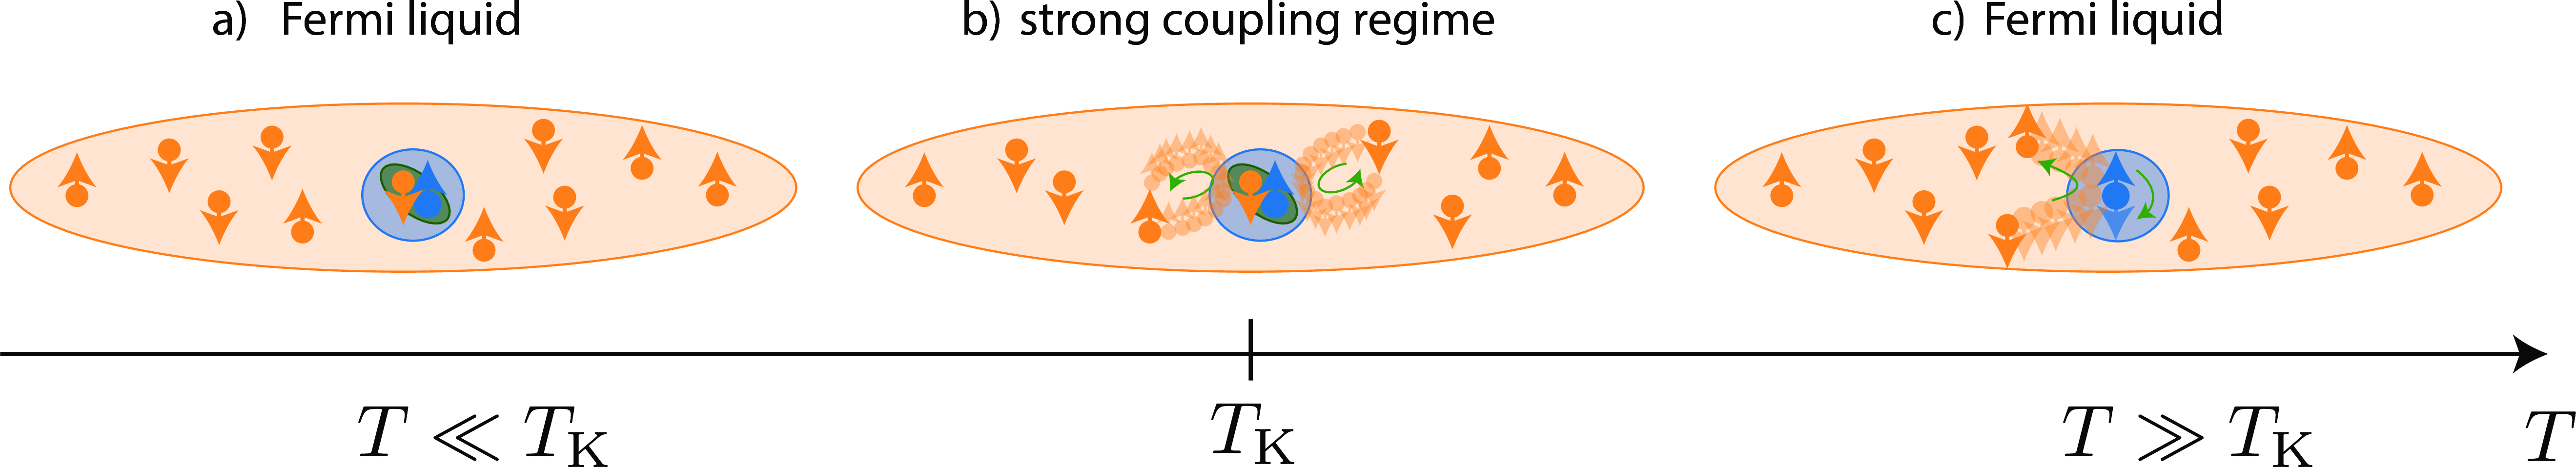
\includegraphics[width=1.00\columnwidth]{figures/SingleChannelKondov3/SingleChannelKondov3}
\caption{{A Fermi~ sea of s = 1/2 particles is~ (orange) is coupled to a localized
impurity (blue), whose only degree of freedom is its spin orientation S
= 1/2. They interact through an anti-ferromagnetic exchange
interaction.~ a) For low temperatures, the interaction leads to the
formation of a spin singlet between a Fermion and the impurity. The high
energy cost of creating an excitation in the region of the impurity
blocks it entirely from the dynamics of the Fermi sea. The Fermions can
now be treated as a Fermi liquid with the impurity region removed. b)
For intermediate temperatures the singlet gets deconfined and virtual
excitations in the impurity region are allowed. As they involve the
neighboring~ Fermions, they can lead to strong interactions between the
previously non-interacting particles. These processes are typically only
describable by non-perturbative techniques. c) For high temperatures,
the interaction with the impurity is~ well described by perturbative
scattering theory and the system is once again well described by a Fermi
liquid.~
{\label{943637}}%
}}
\end{center}
\end{figure}



Several decades after its first discovery in metals, the Kondo effect has been observed in a multitude
of solid-state systems such as quantum dots \cite{Kastner_1998,Cronenwett_1998,Schmid_1998}, carbon nano-tubes \cite{Nyg_rd_2000}, and single molecules \cite{Liang_2002,Park_2002}, confirming the presented equilibrium picture. Dynamical and spatial properties, which would
be observable on time scales of $t \ll \frac{\hbar}{k_B T_K} \sim $ps, remain inaccessible in these solid-state systems.
Such measurement would be however highly desirable, as the Kondo model (and its generalization in form of the Anderson model) is nowadays one of the standard benchmarks for calculations on dynamical and real space properties, where our theoretical understanding is much less complete than in the equilibrium case \cite{Polkovnikov_2011,Bock_2016}. As several aspect of these open questions are captured in the properties of the debated Kondo screening cloud \cite{Park_2013}, it would be of one of the key objectives for any new experiment with ultracold atomic gases to provide precise experimental studies of the Kondo screening cloud and its dynamics with ultracold quantum gases.

\section{Ultracold atoms as experimental platform for impurity models}

The experimental achievement of fabricating gases of ultracold atoms (either Bosons or Fermions) opened the way to study a multitude of fundamental physical phenomena that were otherwise very difficult to realize \cite{Bloch_2008}. They have already proven to be a fantastic tool for the study of several simple impurity problems resulting in numerous intriguing quantum effects.
In the simplest case, the impurities are static. They form a static disorder, which first leads to the well-known diffusion, but can eventually result in Anderson localization via the quantum interference between different diffusive paths \cite{Anderson_1958}. Even sixty years after its initial prediction fundamental questions remain, especially in the higher dimensional case, and ultracold atoms are now a well established tool to investigate this long-standing problem \cite{Billy_2008,Roati_2008,Jendrzejewski_2012,Semeghini_2015}. 

In the slightly more general polaron models, the impurity can move, but has no internal degrees of freedom. The moving impurity is then dressed by a cloud of surrounding particles, leading to the formation of the polaron quasiparticles. Ultracold atomic mixtures are a remarkable tool to investigate the properties of such polarons \cite{Chevy_2010}. In such experiments a small number of atoms of one species act as an impurity. They are immersed in a large Fermi sea or Bose-Einstein condensate, formed by a second species. One can then read out the effective mass \cite{Nascimb_ne_2009} and the binding energy of the impurity \cite{Schirotzek_2009}. With a bosonic bath, these studies have opened the path towards a synthetic quantum vacuum \cite{Rentrop_2016,J_rgensen_2016,Hu_2016}.

\section{On a possible implementation}
Despite this progress, the observation of the Kondo effect remains elusive in the field of ultracold atoms. The impurity should have an internal spin degree of freedom, but remain localized on its site in these systems. Given its fundamental importance, this topic received intense attention recently \cite{Bauer_2013,Nishida_2013,Kuzmenko_2015,Sundar_2016,Gorshkov_2010}. While quantum magnetism of Fermi gases has seen tremendous progress in recent years \cite{Mazurenko_2017}, the Kondo effect seems still out of enormously challenging in existing set-ups \selectlanguage{ngerman}\cite{fölling2017}.

It seems quite natural to implement the Kondo model with a mixture of ultracold atomic gases \cite{Kuzmenko_2015}. A first species, e.g. \textsuperscript{40}K or \textsuperscript{6}Li, would form the Fermi sea. A second species, e.g. \textsuperscript{23}Na, would then be tightly trapped by species-selective optical potentials and from the spin impurity. The spin-exchange could then be mediated by spin-changing collisions, very much in the spirit of our work on dynamical gauge fields \cite{Kasper_2016,Kasper_2017,Jendrzejewski}. We will see where the journey goes from here.

\selectlanguage{english}
\FloatBarrier
\bibliographystyle{plainnat}
\bibliography{bibliography/converted_to_latex.bib%
}

\end{document}

